\section{The {\em paṇḍaka}}



It is clear that the Chinese palace eunuchs cannot be compared to for instance the Hijra from India.

\begin{figure}[!tbp]
  \centering
  \subfloat[Palace eunuchs in ancient China]{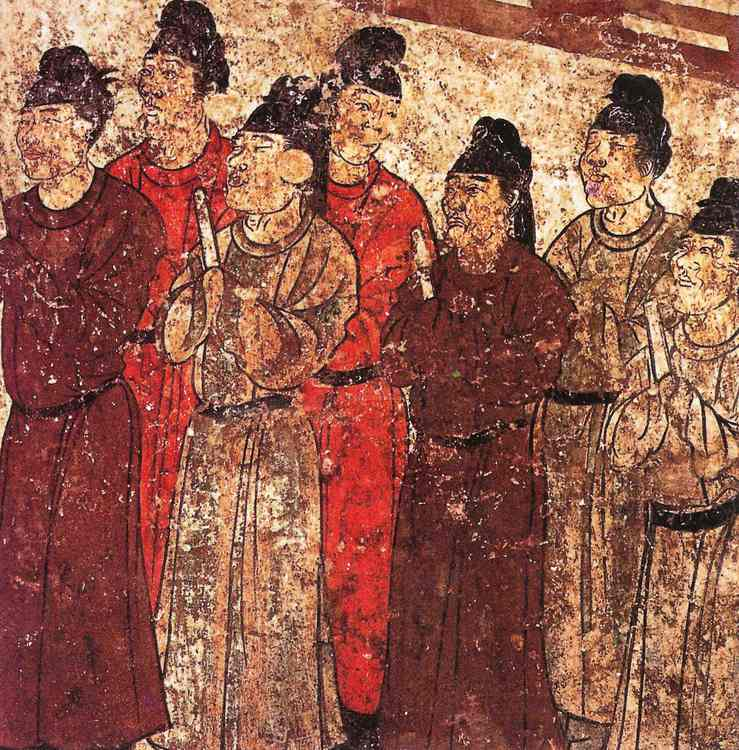
\includegraphics[width=0.4\textwidth]{Eunuchs-in-ancient-China.jpg}}
  \hfill
  \subfloat[Hijra in India]{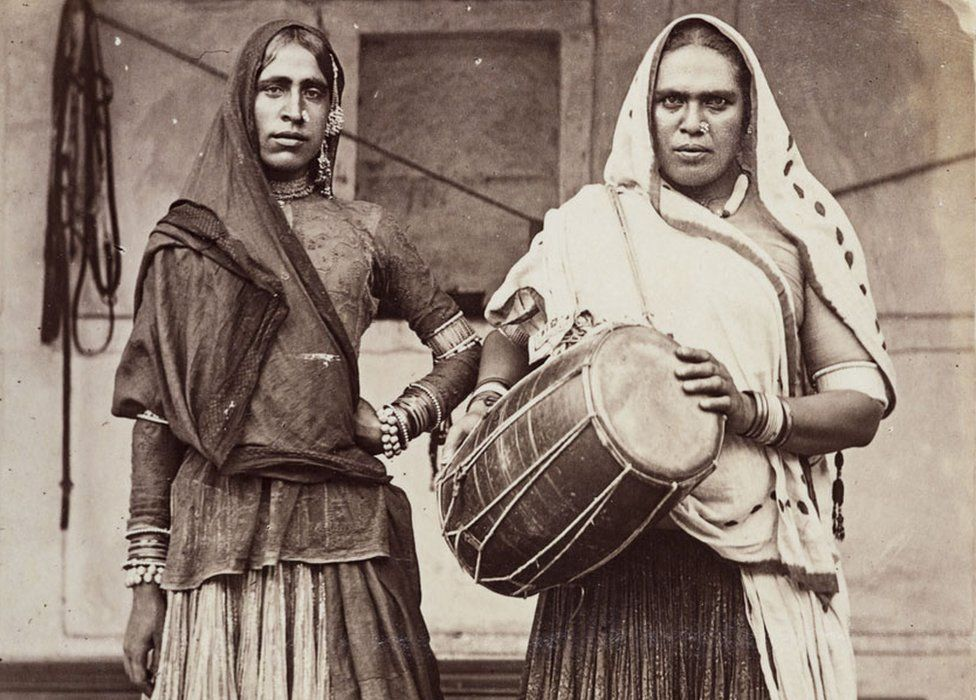
\includegraphics[width=0.4\textwidth]{hijra.jpg}}
\end{figure}

The term 非男非女 (neither male nor female) is only used by the {\em paṇḍaka} to describe himself in the Mahāsaṅghika Vinaya. This could be a literal translation of the term {\em napuṃsaka} as in Vedic India this is an umbrella term of which the {\em paṇḍaka} is a subsection. 

\subsection{Conclusion on {\em paṇḍaka}}
From the above discussion we can conclude that the translation 'eunuch' for {\em paṇḍaka} is 


